\section{Specific Requirements}\label{sec:spec_req}

\subsection{External Interface Requirements}
\subsubsection{User Interfaces}

The application is designed to allow the customer to make a reservation for a certain hour or to register in the current queue of a supermarket. The first time the user opens the app, they are prompted to register for an account: they have to provide their mobile phone number
(Fig. \ref{fig:mockup-welcome}), then they'll receive an SMS with a confirmation code
(Fig. \ref{fig:mockup-login}) to insert.
If the code inserted is the one sent to the phone number inserted in the first screen, the account creation is successful, otherwise the user can ask for a new SMS or go back and enter another phone number.

After a successful registration, the user sees a map (Fig \ref{fig:select-store}) with stores nearby their current location (they might have to allow the app using their location through the OS API), otherwise they can manually search stores by typing an address. The user can narrow their search through filters (Fig. \ref{fig:filters}).
Users can also see shortcuts to stores they have previously marked as ``favorites''.

Upon selecting a store (Fig. \ref{fig:store-details}), the current number of people in queue is shown to the user,
as well as the estimated waiting time in queue. They can choose to enter the queue as soon as possible, or to pick an available time slot. The system also suggests possible alternatives.

If they choose to pick a time slot, they are shown a list of time slots sorted by day (Fig. \ref{fig:select-timeslot}).
Upon confirmation, the user receive a receipt (Fig. \ref{fig:receipt}) with the date and time of their reservation,
and a QR code that they'll need to show when they present themselves at the store.

Should the customer queue for the first available time slot, then they will receive a similar receipt (Fig. \ref{fig:queue-ticket}),
that has a countdown of the time remaining in queue before their visit.

In either case, users can cancel their reservations/queue from the receipt screen.

\begin{figure}[H]
    \caption{Mock-up of the Application User Interface}
    \subfloat[Welcome Screen]{
        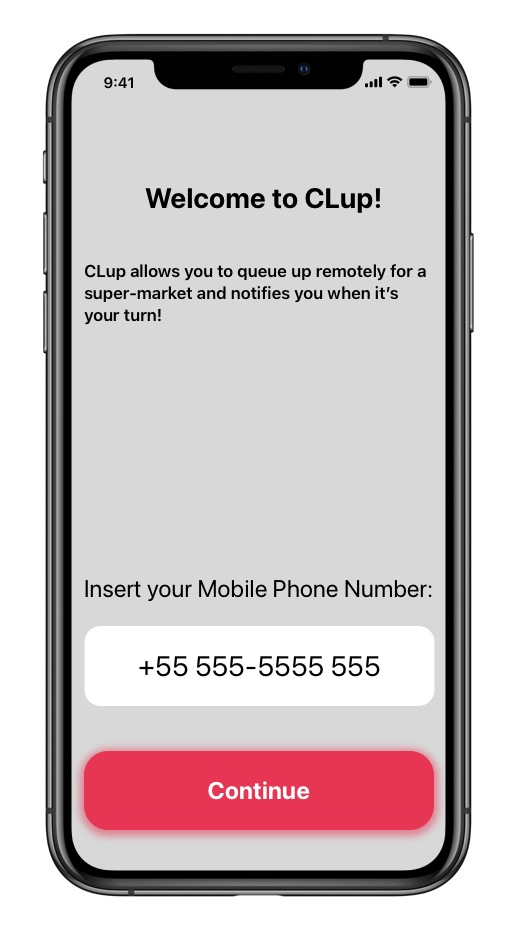
\includegraphics[width=0.25\textwidth]{images/mockup/welcome-screen.png}
        \label{fig:mockup-welcome}
    }
    \subfloat[Confirm Login]{
        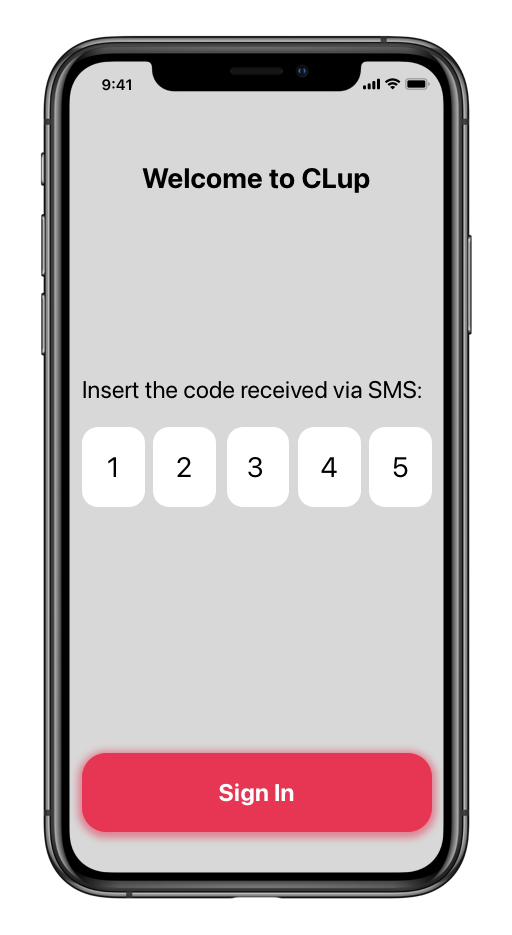
\includegraphics[width=0.25\textwidth]{images/mockup/confirm-login.png}
        \label{fig:mockup-login}
    }
    \subfloat[Select Store]{
        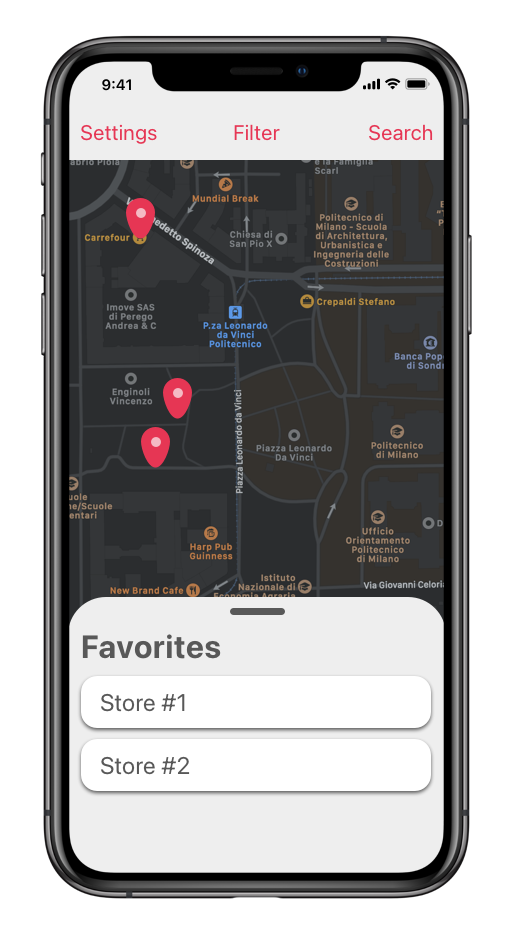
\includegraphics[width=0.25\textwidth]{images/mockup/map-select.png}
        \label{fig:select-store}
    }
    \subfloat[Filters]{
        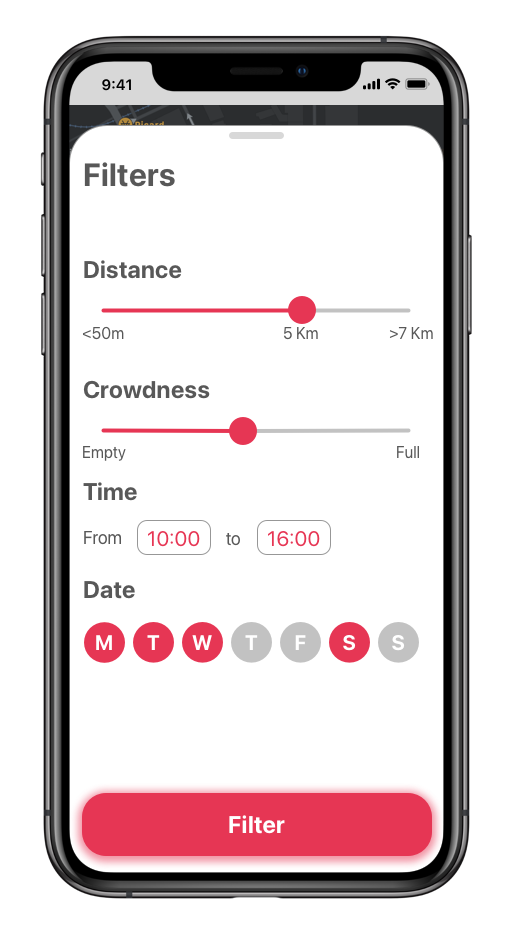
\includegraphics[width=0.25\textwidth]{images/mockup/filters.png}
        \label{fig:filters}
    }
    \newline
    \subfloat[Store Details]{
        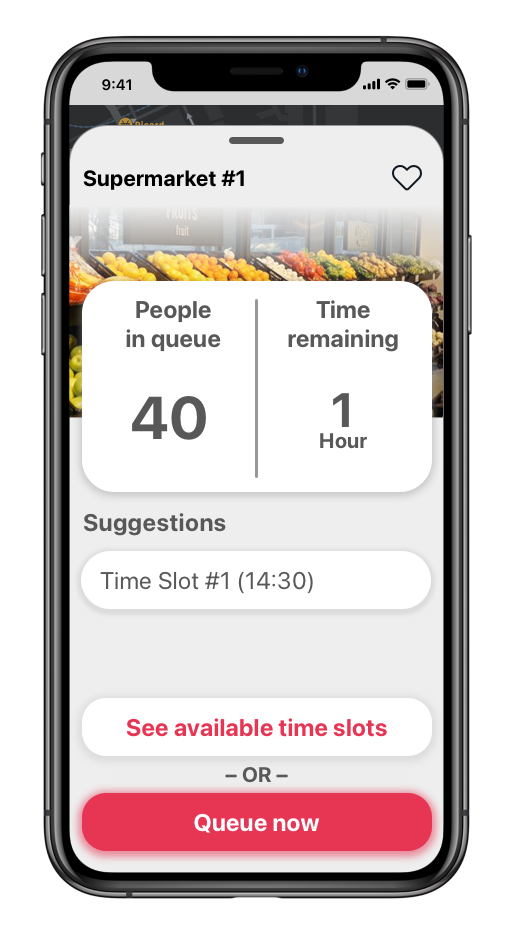
\includegraphics[width=0.25\textwidth]{images/mockup/store-detail.png}
        \label{fig:store-details}
    }
    \subfloat[Select Timeslot]{
        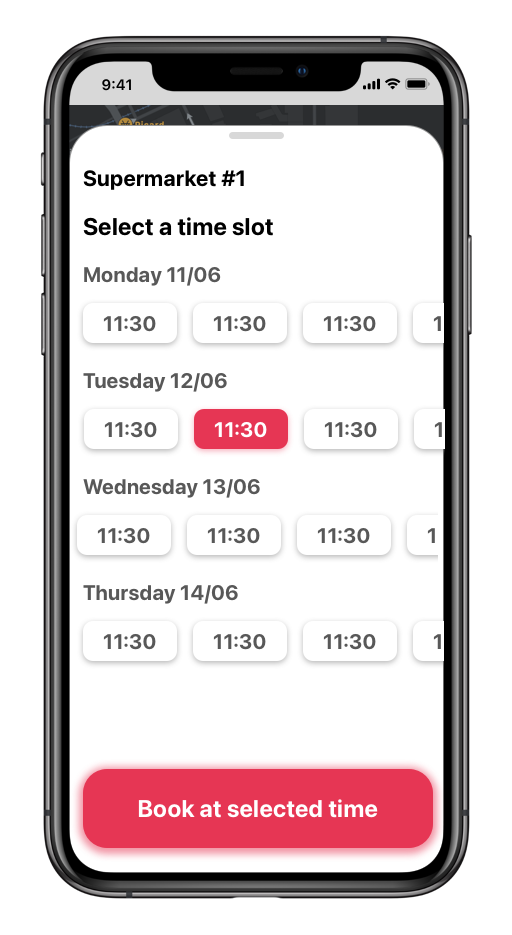
\includegraphics[width=0.25\textwidth]{images/mockup/time-slots.png}
        \label{fig:select-timeslot}
    }
    \subfloat[Reservation Receipt]{
        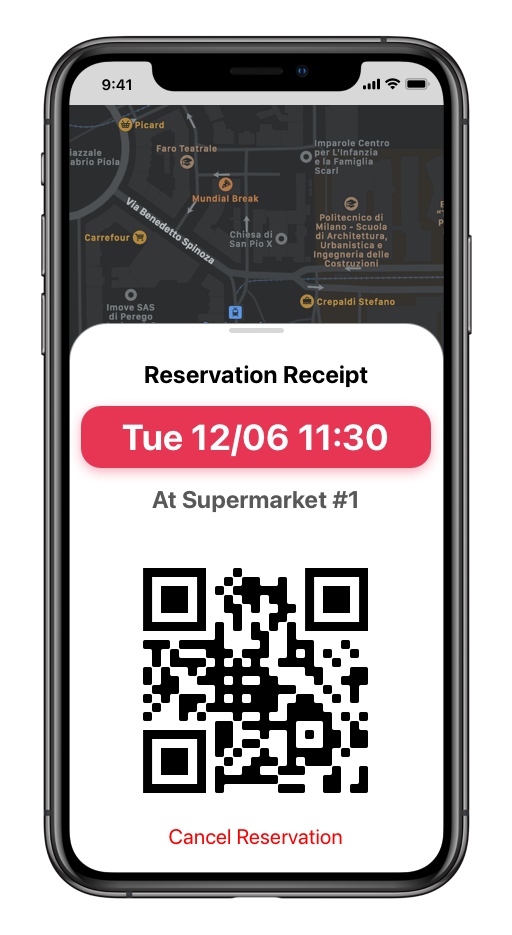
\includegraphics[width=0.25\textwidth]{images/mockup/receipt.png}
        \label{fig:receipt}
    }
    \subfloat[Queue Ticket]{
        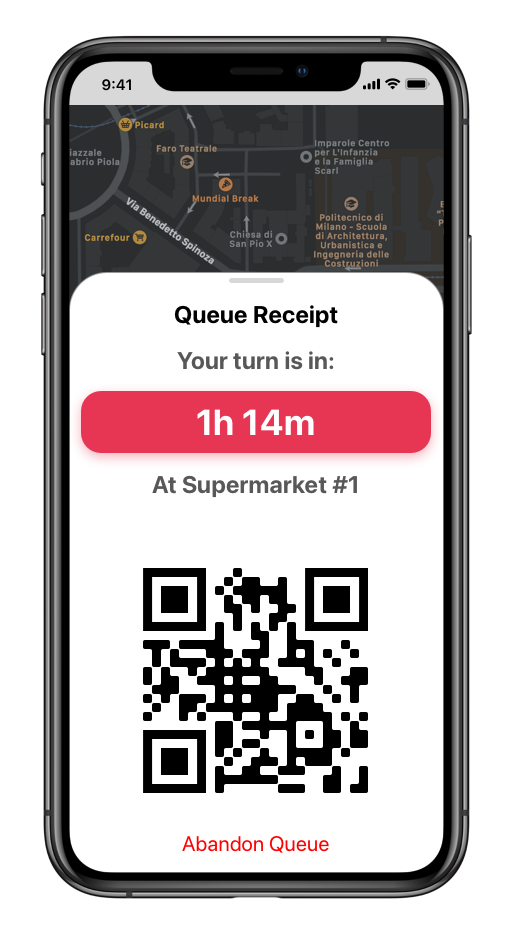
\includegraphics[width=0.25\textwidth]{images/mockup/queue-ticket.png}
        \label{fig:queue-ticket}
    }
\end{figure}


\subsubsection{Hardware Interfaces}

An interactive totem (Fig. \ref{fig:totem}) with a touchscreen display should be made available at each store entrance, to account for Customers that do not have an Internet connected device at their disposal.
The totem is connected to Internet or the store local network.
It mirrors the key features of the web application, but it doesn't require the customer to
authenticate. Customers is able to enter the queue, but they won't be able to
be notified of possible changes/delays. The reservation receipt is printed and the customer must keep it until they're
admitted to the store, otherwise they won't be able to enter.
The store will also have a monitor showing the current status of the queue and the users in queue who have to enter the store.
\begin{figure}[H]
    \centering
    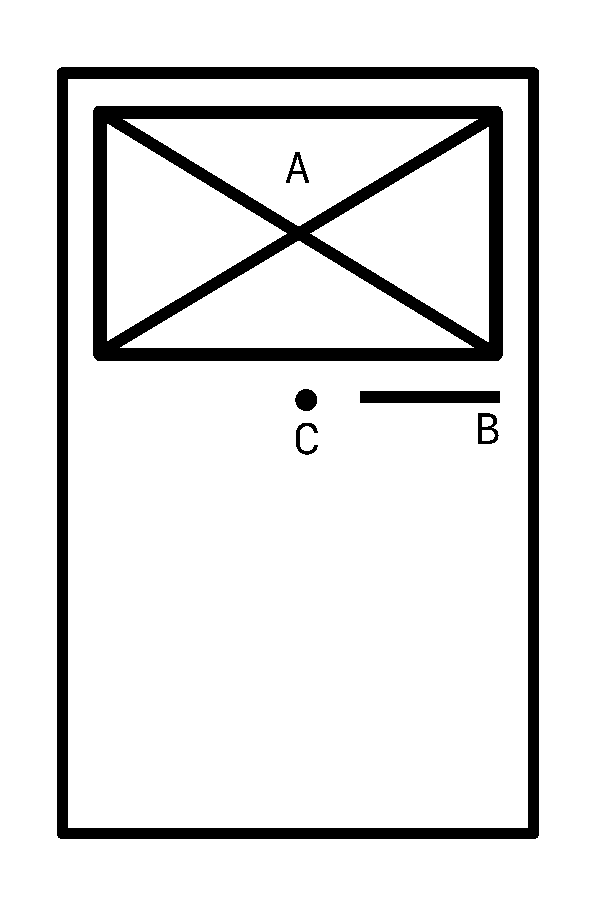
\includegraphics[width=0.25\textwidth]{images/totem.pdf}
    \caption{The totem interface: (A) is the touchscreen display,
    (B) is where the printed ticket is emitted, (C) is a proximity sensor that wakes the
    totem when a client is nearby.}
    \label{fig:totem}
\end{figure}

\subsubsection{Software Interfaces}
In order to provide its full functionality to all users, the system will make use of the following software interfaces (APIs):
\begin{itemize}
    \item \textbf{Maps}: to implement the functionality allowing the Users to look for a store the system will interface with a digital map service. Store Managers will be able to register on the map the position of their store.
    \item \textbf{Geolocalization}: geolocalization through GPS (when available) or other means (cellular, WI-FI or IP location) will be used in the web app and in the mobile app in order to show the User their current position and help them find a nearby store.
    \item \textbf{Mobile OS Notification Service}: notifications will be sent to warn and update Users in real time about their Reservations (if any) and the status of the Virtual Line (if it is joined).
    \item \textbf{SMS service}: an SMS with a secret code will be sent to the user upon login in order to verify their identity through a third party service.
\end{itemize}

\subsubsection{Communication Interfaces}
The backend of the system will expose a unified REST compliant API to communicate with all clients using HTTPS and TCP/IP.
The User will need a working Internet connection as well as cellular network upon login.
The Totem will be provided with WiFi, wired or cellular connectivity, depending on the physical constraints of each store.

\subsection{Functional Requirements}
Definition of use case diagrams, use cases and associated
sequence/activity diagrams, and mapping on requirements

\begin{enumerate}[label={[R\arabic*]}]
    % Users
    \item Allow a User to sign up for an Account after providing a mobile phone number.
    \item Allow a Registered User to find Stores nearby a specified location.
    \item Allow a Registered User to filter out stores based on available timeframes, days and distance.   
    \item Allow a Registered User to get in the virtual line at a specified store.
    \item Allow a Totem User to get in the virtual line of the store where the totem is installed.
    \item Allow a Registered User to preview an estimate of the queue time.
    \item Allow a Registered User to book one visit to a specific store.
    \item Allow a Registered User to cancel their reservation.
    \item Allow a Registered User to leave the virtual queue.
    \item Allow a Registered User and a Totem User to retrieve a scannable QR Code/Barcode that they must present in order to be granted access to a store.

    % Store
    \item The System notifies the Users affected by delay.
    \item The System cancels User reservations in case of a major delay.
    \item The System enforces the limits on the allowed number of concurrent Customers inside a store by restricting the access at the entry points (for example, automatic doors or turnstile).
    \item The System grants a User with a reservation access only within a short time (set by the manager) after the User's time of reservation.
    \item Allow System Managers to set the division of the maximum number of people allowed between the normal queue, the priority queue for people with special needs and the book a visit slot capacity.    
    \item The System calculates the average shopping time by recording every time a user enters and exits the store.
    
    % System Managers
    \item Allow System Managers to set a limit to the people allowed into the store at a time.
    \item Allow System Managers to choose the frequency and size of the time slots.
    \item Allow System Managers to know the average time spent in the store.
    \item Allow System Managers to know the current and past number of people in the store.
    \item Allow System Managers to check the current status of the queue and of the time slots.
    
\end{enumerate}

\begin{center}
    \begin{tabular}{ |c||c|c| }
        \hline
        \textbf{Goal} & \textbf{Requirements} & \textbf{Assumptions} \\
        \hline
        G1 & R1, R2, R3, R4, R5, R6, R7, R10, R13, R14, R17 & D1, D2, D3, D5 \\ % G: Avoid crowds
        \hline
        G2 & R15 & D3, D4, D5 \\ % G: Priority Access
        \hline
        G3 & R6, R7, R11, R12 & D2, D5, D6\\ % G: Save time
        \hline
        G4 & R10, R13, R14, R15, R17, R18 & D1, D3, D4 \\ % G: Set Max No. of Customers and other parameters
        \hline
        G5 & R16, R19, R20, R21 & D1, D3, D4, D5, D6 \\ % G: Monitor and Statistics
        \hline
    \end{tabular}
\end{center}

\begin{center}
    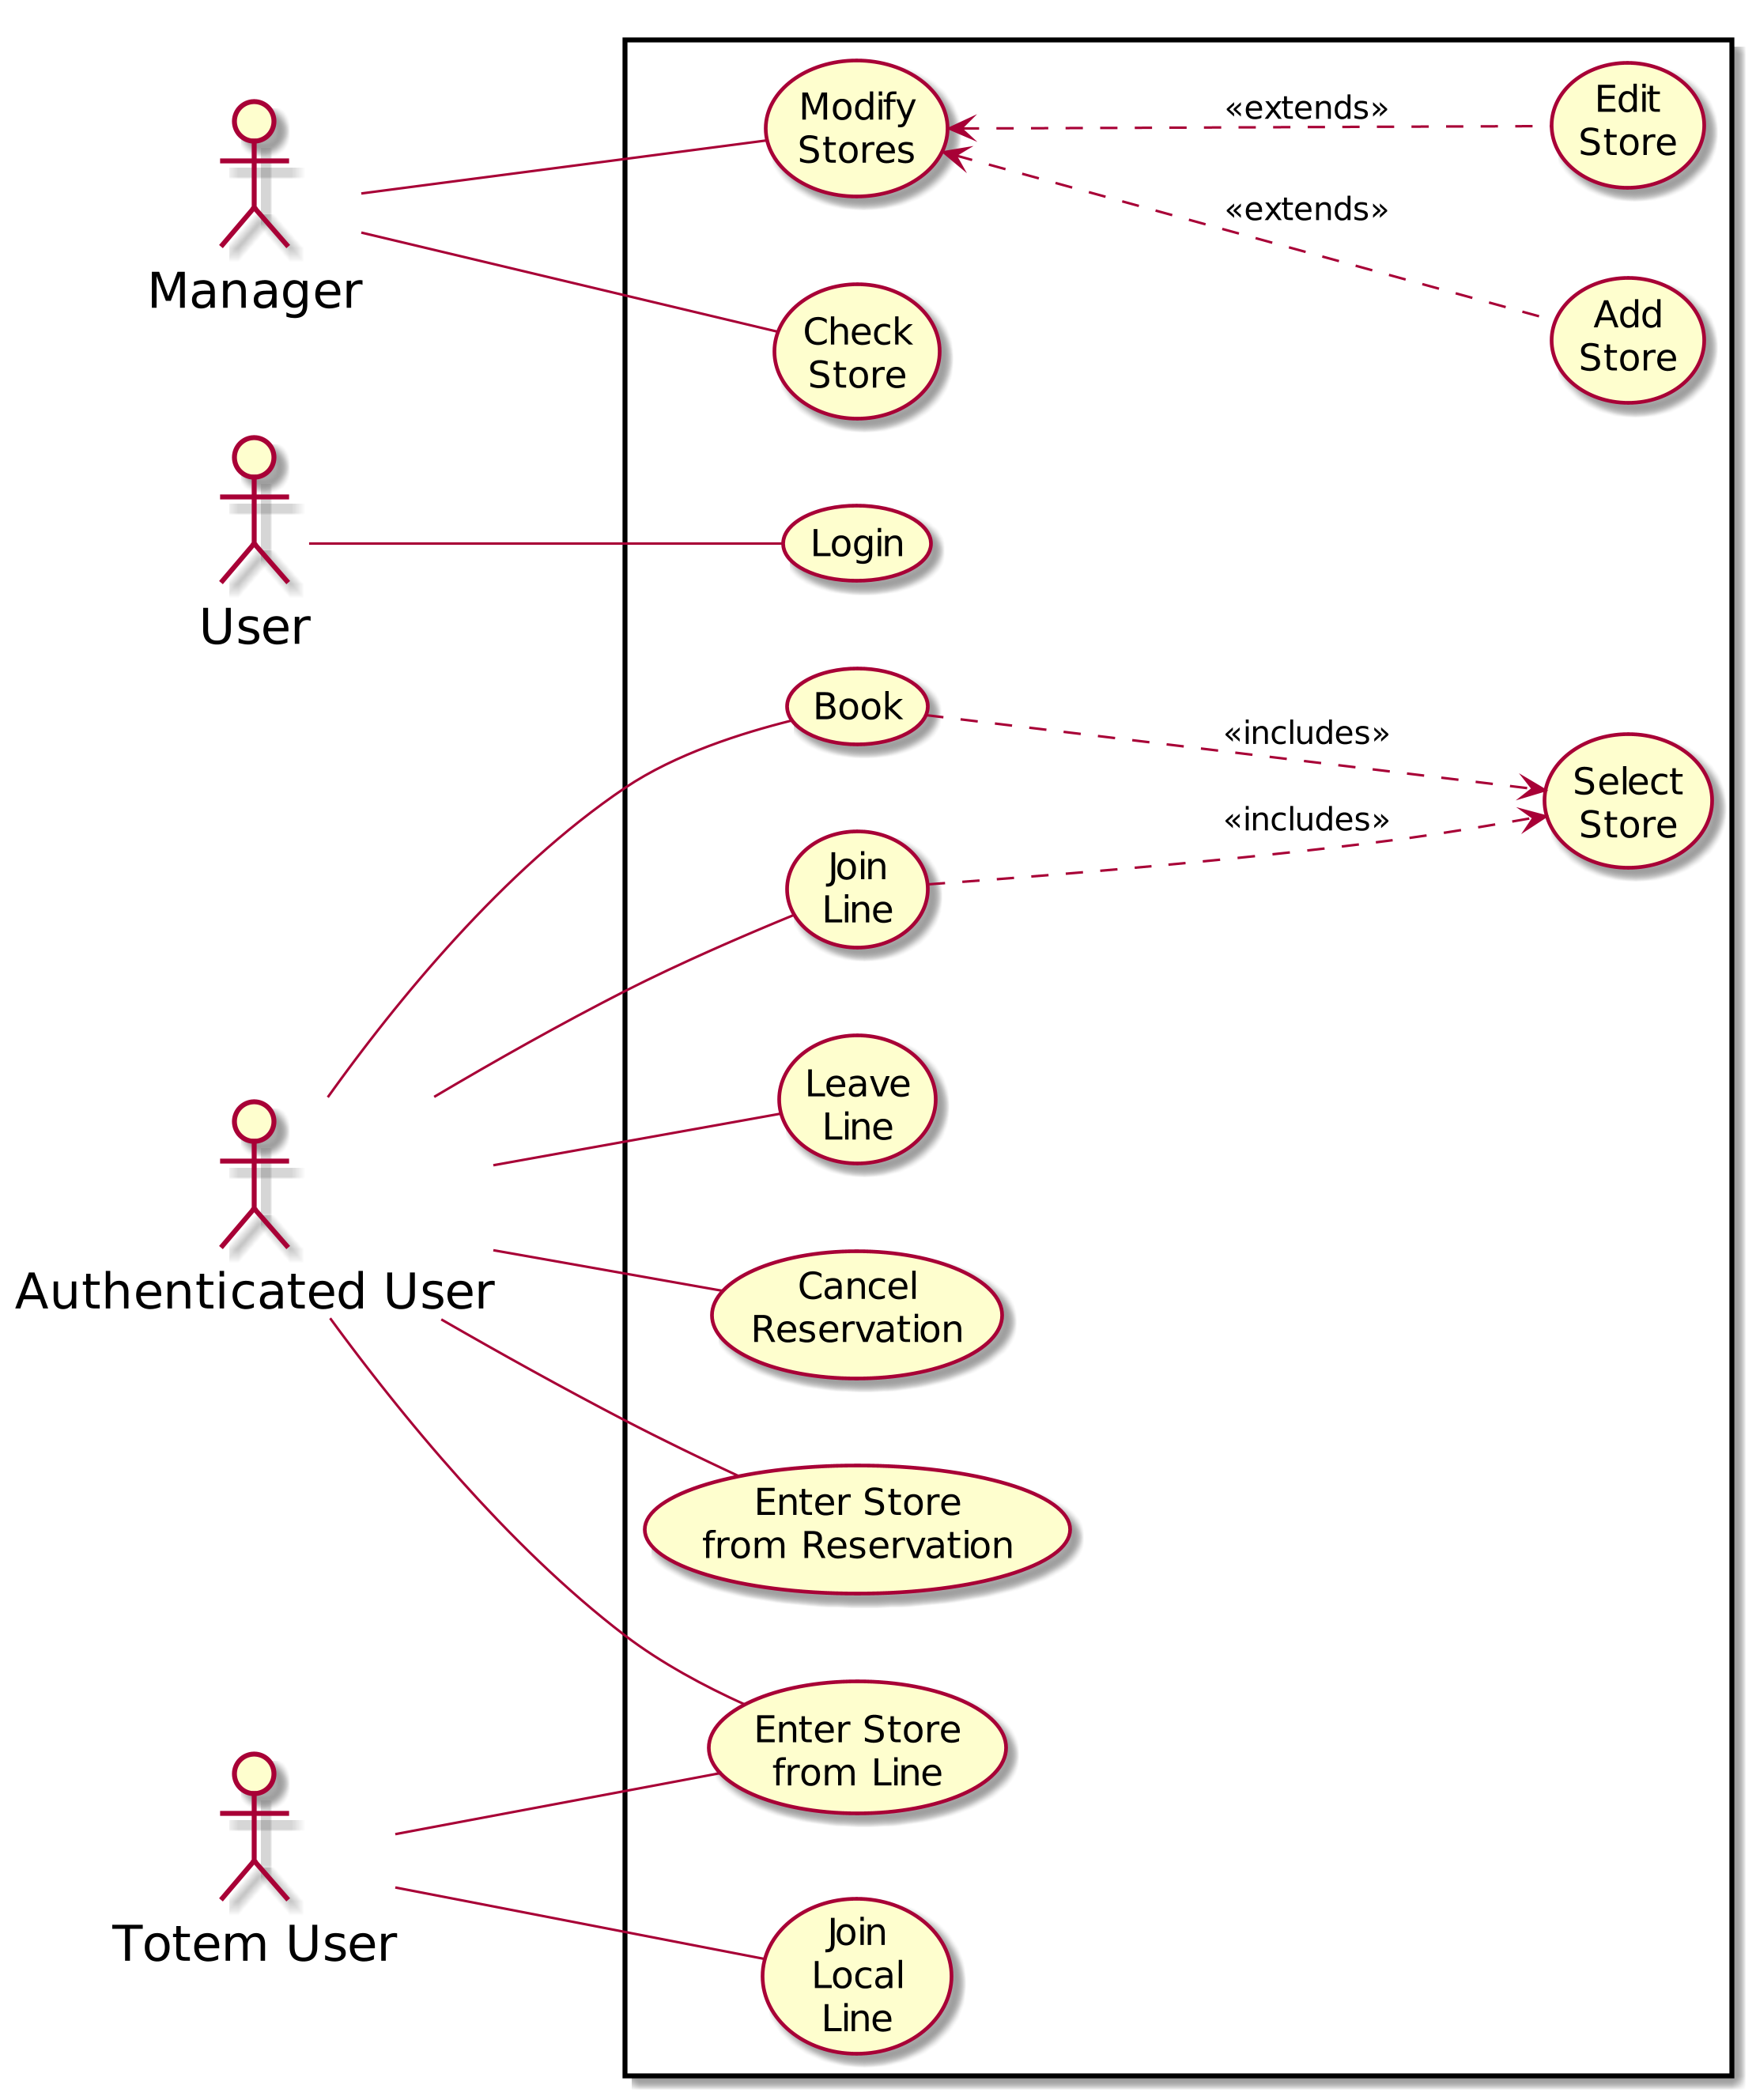
\includegraphics[width=\textwidth]{uml/usecase.png}
\end{center}


%----------------------------------------------------------------------------------------------------
%                                           USE CASES
%----------------------------------------------------------------------------------------------------

\usecase
{Login}
{Customer}
{The Customer has installed the application on their device.}
{
    \begin{enumerate}
        \item The Customer opens the application.
        \item The Customer may read Privacy Policy and the Terms of Service by clicking on the respective links. If they create an account, it's implied that they accept them.
        \item The Customer enters their mobile phone number and taps ``Continue''.
        \item The Customer enters the received token via SMS and taps ``Sign In''.
    \end{enumerate}
}
{The Customer is now logged-in and they may utilize the application.}
{
    \begin{itemize}
        \item The Customer inputs invalid data.
        \item The Customer doesn't fill the required data.
    \end{itemize}
}
{
    When an exception occurs, the user is informed by a human-readable message.
    In case the user thinks the SMS hasn't been sent/received, they can ask the system for a new token.
}

\usecase
{Select Store}
{Authenticated User}
{An authenticated User, with no pending reservation, opens the application.}
{
        \begin{enumerate}
            \item (Optional) The Authenticated User applies some filters to restrict the available stores.  
            \item The System provides the user with a list of the supermarkets near him.
            \item The Authenticated User is able to see a preview of the number of people in queue and the estimated waiting time. 
            \item The user selects the desired store. 
            \item The user is now able to see full screen the waiting time and the number of people in queue (and possibly other stats on the store), and is given the possibility to join the line or make a reservation if time slots are available.  
        \end{enumerate}
}
{
    The Authenticated User has selected a store that suits their need, and is given the possibility to join the line or make a reservation. 
}
{
    \begin{itemize}
        \item There are no open stores in the area. 
        \item There are no stores in the area. 
    \end{itemize}
}
{
    When an exception occurs the users is promted to check the application again later. 
}

\usecase
{Join Queue}
{Authenticated User}
{Authenticated User selects a Supermarket in the application}
{
        \begin{enumerate}
            \item The Authenticated User pushes the "Queue Now" button.
            \item The system provides the Queue Receipt with the generated QR code and the estimated time remaining.
        \end{enumerate}
}
{
    The customer is now in the queue waiting for their turn, and will receive notifications about the state of the queue.
}
{}
{}


\usecase
{Book}
{Authenticated User}
{Authenticated User selects a Supermarket in the application}
{
        \begin{enumerate}
            \item One of the following path:  
            \begin{enumerate}
                \item The Authenticated User pushes the "Make a Reservation" button.
                \begin{itemize}
                    \item The user chooses a suitable time among the available ones.
                \end{itemize}
                \item The Authenticated User selects the less crowded slot proposed by the application.
            \end{enumerate}
            \item The system provides the Reservation Receipt with the generated QR code.
        \end{enumerate}
}
{
    The customer has now a pending reservation.
}
{}
{}


\usecase
{Leave Queue}
{Authenticated User}
{Authenticated user enters the home page of the application and is currently in Line.}
{
    \begin{enumerate}
        \item The Authenticated User clicks the "Leave Current Queue" button.
        \item The Authenticated User confirms the selection.
    \end{enumerate}
}
{
    The customer has now left the queue.
}
{}
{}

\usecase
{Cancel Reservation}
{Authenticated User}
{Authenticated user enters the home page of the application and has a pending Reservation.}
{
    \begin{enumerate}
        \item The Authenticated User clicks the "Cancel Current Reservation" button.
        \item The Authenticated User confirms the selection.
    \end{enumerate}
}
{
    The customer has now canceled the reservation.
}
{}
{}


\usecase
{Join Local Queue}
{Totem User}
{A user approaches the totem in front of a store while the store is open.}
{
    \begin{enumerate}
        \item The user clicks the button appearing on screen.
        \item The totem prints a ticket containing a QR code and the estimated waiting time.
    \end{enumerate}
}
{
    The user is now in queue.
}
{}
{}


\usecase
{Enter Store from Queue}
{Registered User, Totem User}
{A user is in Queue.}
{
    \begin{enumerate}
        \item The user waits until the ID on their ticket comes up on the monitor at the store or until a notification on the app appears.
        \item The user enters the store by letting the totem read their QR code, shops, and exits the store.
    \end{enumerate}
}
{
    The user has shopped.
}
{
    \begin{itemize}
        \item There is a major delay in the store. 
        \item The time remaining to wait in the queue exeeds the opening hours of the store. 
    \end{itemize}
}
{
    When an exception occurs, the user is asked to leave, through a notification on the app or at the store at the monitor. 
}

\usecase
{Enter Store from Reservation}
{Authenticated User}
{User has a reservation}
{
        \begin{enumerate}
            \item The user reaches the store at the specified time.
            \item The user enters the store by letting the totem read their QR code, shops, and exits the store.
        \end{enumerate}
}
{
    The user has shopped.
}
{
    \begin{itemize}
        \item There is a major delay.
        \item The user does not reach the store in time.
    \end{itemize}
}
{
    When there is a major delay the reservation is either postponed with the confirmation of the user or automatically cancelled, depending on the estimated waiting time.
    If the user does not reach the store in time the reservation is automatically canceled.
}

\usecase
{Edit Store}
{Manger}
{The manager knows their own credentials for the web panel.}
{
    \begin{enumerate}
        \item The manager opens the apposite web portal.
        \item The manager inserts their credentials and confirm the login.
        \item The manager chooses from a menu the operation they want to perform.
        \item The manager edits the parameters of the system.
    \end{enumerate}
}
{
    The new parameters are applied.
}
{
    \begin{itemize}
        \item The Manager inputs the wrong credentials.
    \end{itemize}
}
{
    In case of a failed login, the Manager is informed by the System on how to retrieve their credentials, had they been forgotten.
}

\usecase
{Add Store}
{Manger}
{The Manager is logged into the web panel.}
{
    \begin{enumerate}
        \item The manager chooses from a menu the option to add a new store.
        \item The manager enters the details of the new store in a form.
        \item The manager submits the form.
    \end{enumerate}
}
{
    A new store is added to system.
}
{
    \begin{itemize}
        \item The store can't be added.
    \end{itemize}
}
{
    In case of exceptions, the manager is informed by a human-readable message.
}


\subsubsection{Sequence Diagrams}

\todo{Add another one?}

\begin{figure}[H]
    \centering
    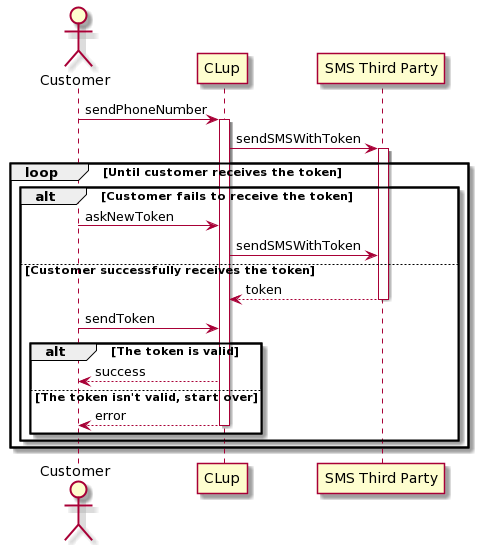
\includegraphics[width=1\textwidth]{uml/login.png}
    \label{fig:seqdiag-login}
    \caption{Login Sequence Diagrams}
\end{figure}

\begin{figure}[H]
    \centering
    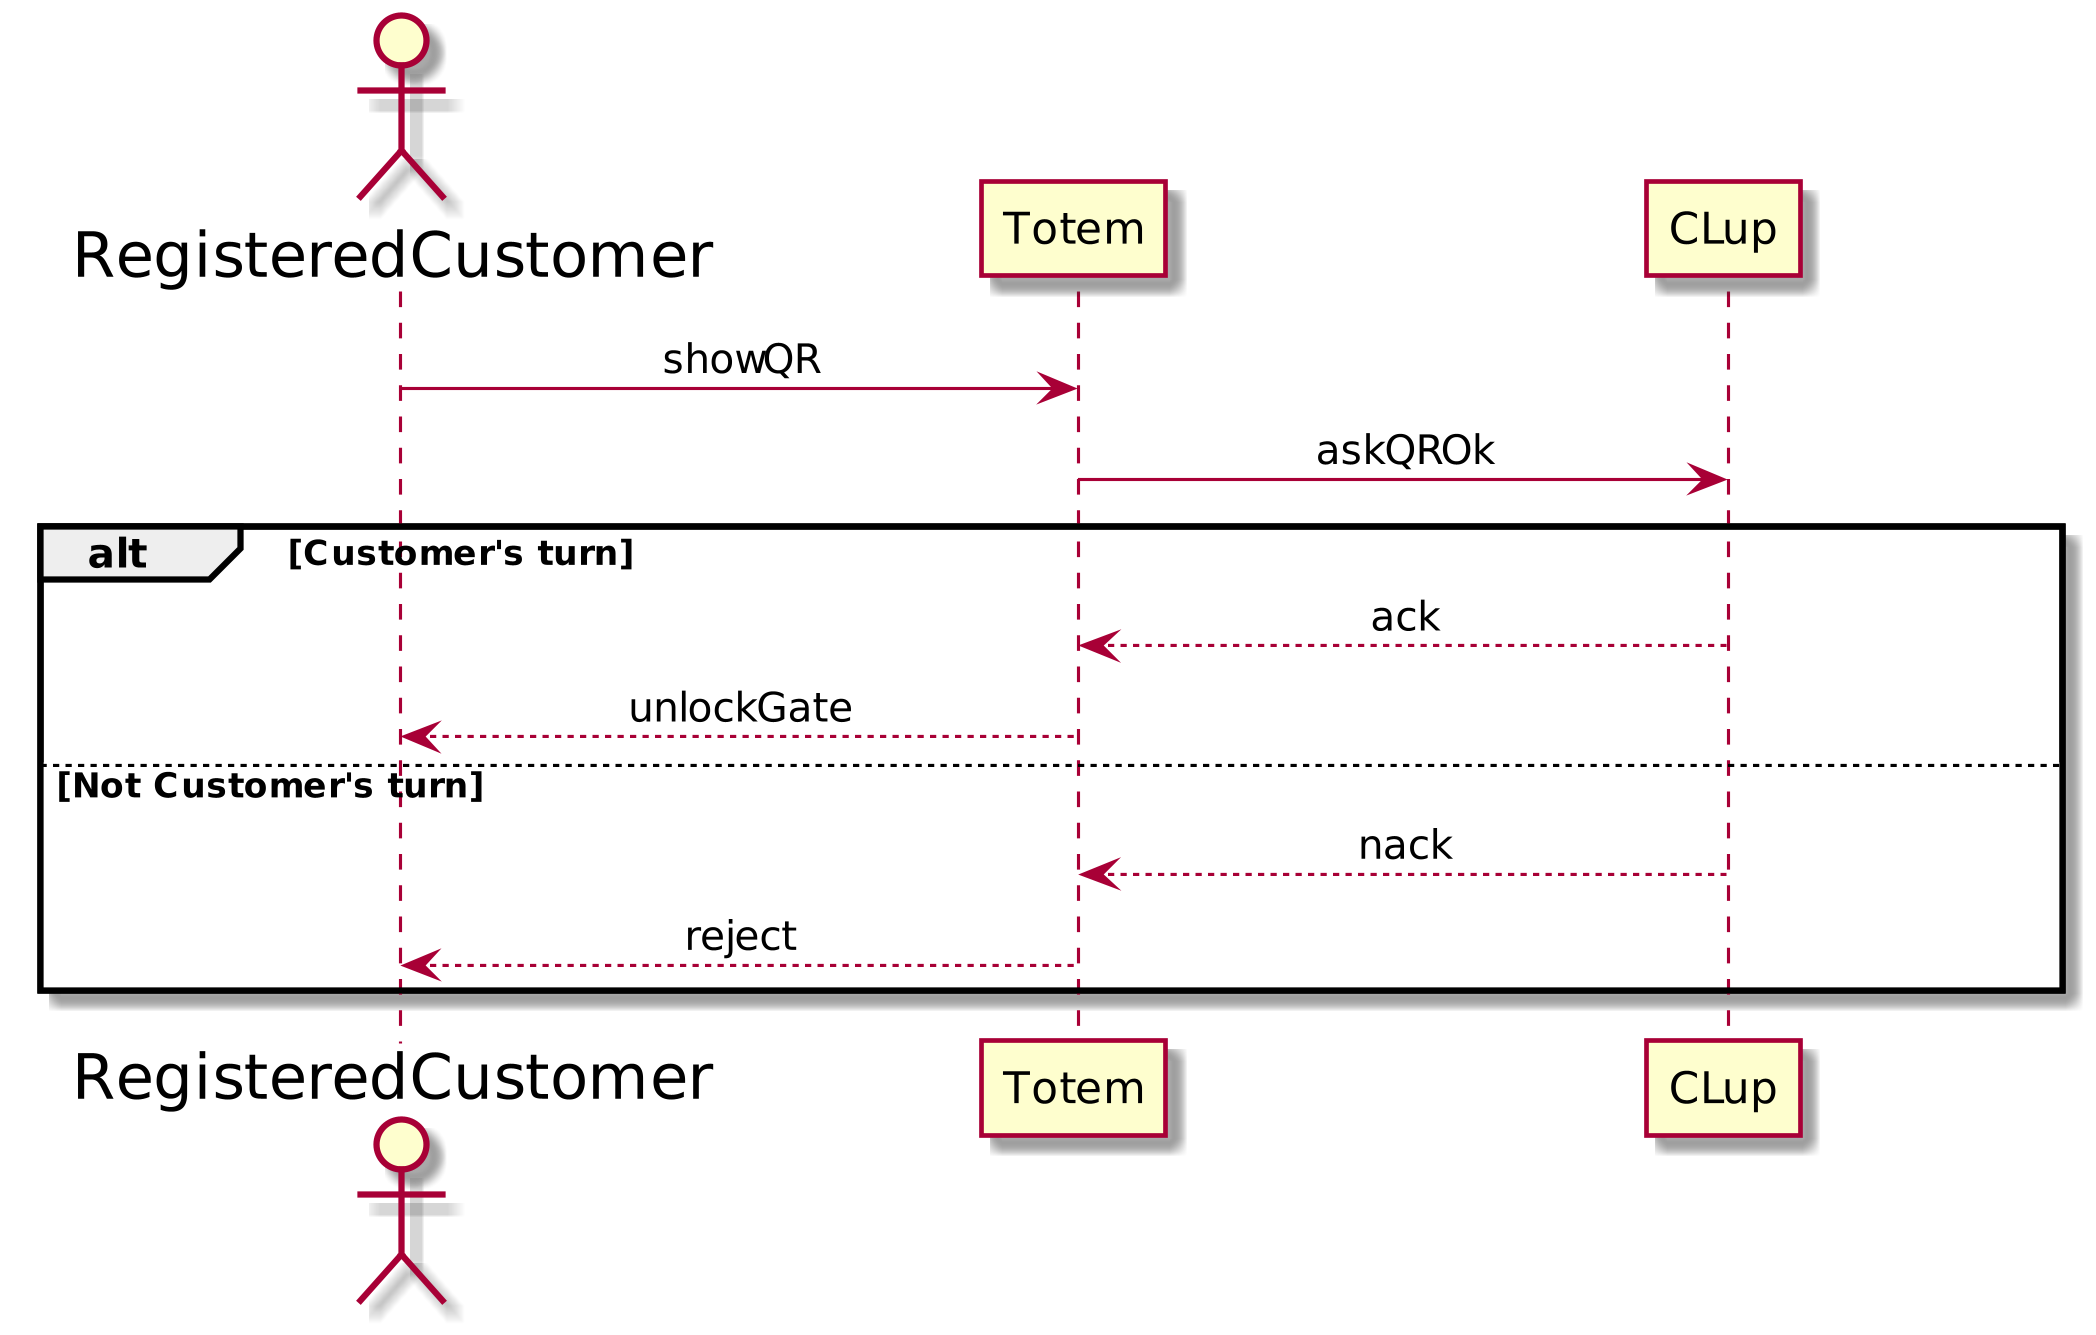
\includegraphics[width=1\textwidth]{uml/enter_queue.png}
    \label{fig:seqdiag-enter_queue}
    \caption{Enter Store from Queue Sequence Diagram}
\end{figure}

\begin{figure}[H]
    \centering
    \begin{minipage}[b]{0.4\textwidth}
      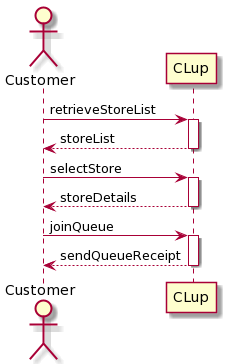
\includegraphics[width=\textwidth]{uml/join_queue.png}
      \label{fig:seqdiag-join-queue}
      \caption{Join Queue}
    \end{minipage}
    \hfill
    \begin{minipage}[b]{0.4\textwidth}
      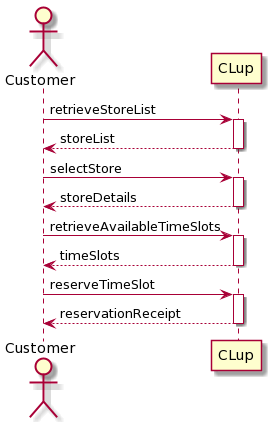
\includegraphics[width=\textwidth]{uml/reserve_timeslot.png}
      \label{fig:seqdiag-reserve-timeslot}
      \caption{Reserve Timeslot}
    \end{minipage}
\end{figure}




\subsection{Performance Requirements}
The system backend needs to handle a fair amount of customers, but little amount of data. It needs to be scalable, capable of load-balancing and reactive in order to notify customers on time. Protection against denial of service attacks would be necessary.
Since each store chain has to deploy its own version of this system, they should estimate server resources based on the average amount of customers visiting their stores.
Client-side and web applications must be responsive, fluid and handle correctly asynchronous interactions with the server (especially when the connection quality is bad), in order to provide the best experience possible to the end user.


\subsection{Design Constraints}
% Specify constraints on the system design imposed by external standards, regulatory requirements or
\subsubsection{Standards Compliance}
The system shall keep track of interactions with the system by the customers (i.e. joining the queue, entering the store, exiting the store).
The data should be named accordingly to this document (RASD) and the Design Document (DD).
All users sensible data shall be handled according to existing regulations, such as the GDPR.

\subsubsection{Hardware Limitations}
\todo{Check if it's ok, I didnt find much on this section in the IEEE ref}
\begin{itemize}
    \item Mobile Application
    \begin{itemize}
        \item iOS or Android smartphone
        \item Cellular data connection
        \item WiFi
        \item GPS
    \end{itemize}
    \item Web Application
    \begin{itemize}
        \item Internet connection
        \item Computer/Tablet with a display
        \item Major recent browser release (Firefox or WebKit based browser)
    \end{itemize}
    \item Backend
    \begin{itemize}
        \item Scalable webserver
        \item Database Management System
    \end{itemize}
\end{itemize}

% \subsubsection{Any Other Constraint}
\subsection{Software System Attributes}
\subsubsection{Reliability}
The system infrastructure should have the lowest MTTR reasonably achievable; should the system need maintenance, it should take place outside store opening hours or during the weekend. It's important to prevent data loss through redundant storage methods.

\subsubsection{Availability}
The whole system doesn't need to be functional 24/7, but certain parts (i.e. backend for the web and mobile app) must be functional at all times to allow user to book a visit at any hour of the day; the totems can be powered off after a certain hour to save energy. The managers web portal should not be heavy on computing resources therefore it's feasible to keep it online all the time.

\subsubsection{Security}
To protect customers sensible data (i.e. phone number, visits to stores, location) the system should collect in first place the required minimum data possible, and store them in an encrypted database. The connections to the system should follow modern standard protocols (HTTPS over TLS) and be encrypted as well. Since managers must log in with username and password, those data should be encrypted and the password salted and hashed.

\subsubsection{Maintainability}
All the code produced should be well commented and tested. The system structure should provide the ability to deploy updates in the backend without the user noticing it. 
System components should be created to be as modular as possible. 
Mobile applications can be updated through their OS app store to release new features and fixes.

\subsubsection{Portability}
The application must be available on major mobile OSs (Android and iOS) targeting at least the current release, even though the previous would be ideal.
The web application must run at least on the most recent browsers, but browser support can be limited.
It would be a smart choice to reuse most of the codebase across mobile and web by using cross platform tools.